\begin{appendices}
\renewcommand\chaptername{Appendix}
\chapter*{Appendix}
\addcontentsline{toc}{chapter}{Appendix}
\label{ch:appendix}
\renewcommand{\thesection}{A.\arabic{section}}
\renewcommand{\thefigure}{A.\arabic{figure}}
\setcounter{figure}{0}
\setcounter{section}{0}
\markboth{APPENDIX}{APPENDIX}

We use the following notation for groups:

\begin{itemize}
\item $D_n$ - dihedral group of order $n$,
\item $S_n$ - symmetric group of degree $n$,
\item $C_n$ - cyclic group of order $n$,
\item $G x H$ - direct product of groups $G$ and $H$
\end{itemize}

\section{Partial automorphism monoid of minimal asymmetric graph X1}

\begin{figure}[H]
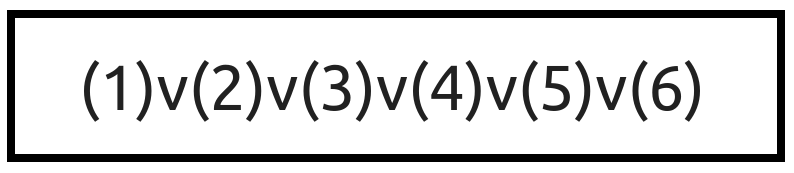
\includegraphics[scale=0.12]{images/x1/x1_6v_6e.png}
\caption{$\mathcal{D}$-class of induced subgraph with 6 vertices and 6 edges.}
\end{figure}

\begin{figure}[H]
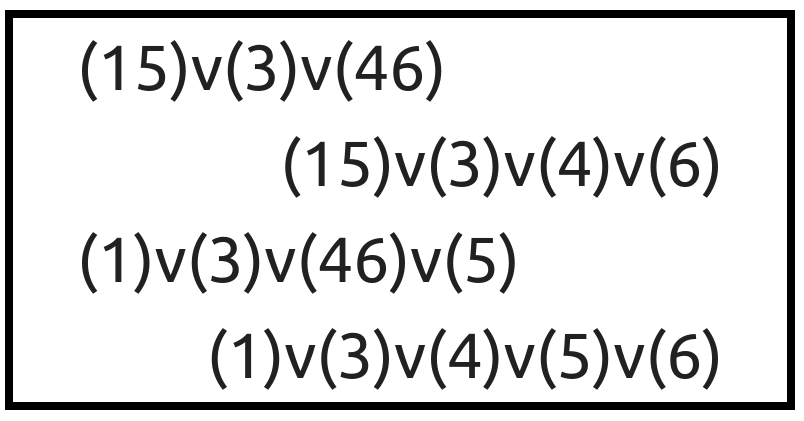
\includegraphics[scale=0.1]{images/x1/x1_5v_3e_2.png}
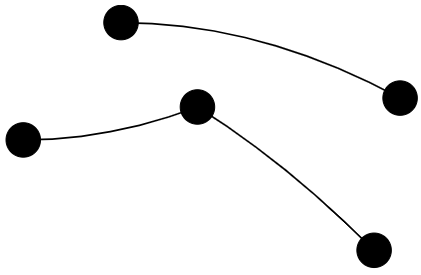
\includegraphics[scale=0.15]{images/x1/x1_5v_3e_2_vis.png}
\caption{$\mathcal{D}$-class of induced subgraph with 5 vertices and 3 edges (group C2xC2).}
\end{figure}

\begin{figure}[H]
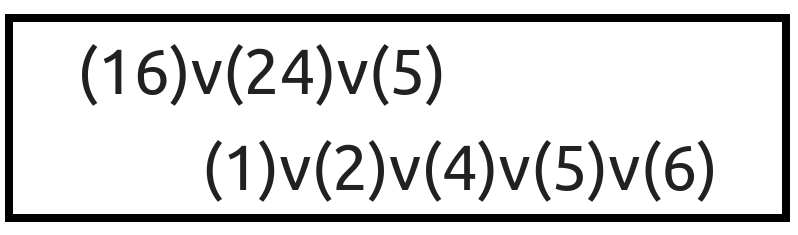
\includegraphics[scale=0.12]{images/x1/x1_5v_3e.png}
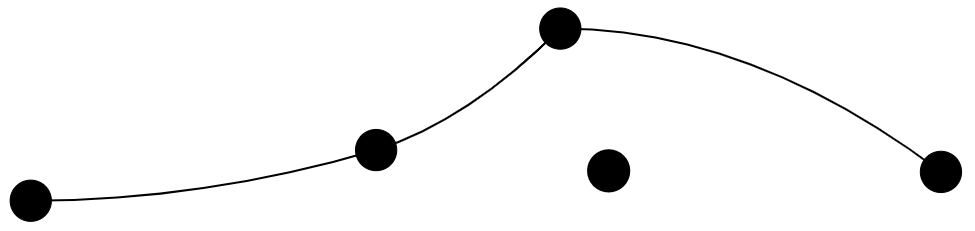
\includegraphics[scale=0.12]{images/x1/x1_5v_3e_1_vis.png}
\caption{$\mathcal{D}$-class of induced subgraph with 5 vertices and 3 edges (group C2).}
\end{figure}

\begin{figure}[H]
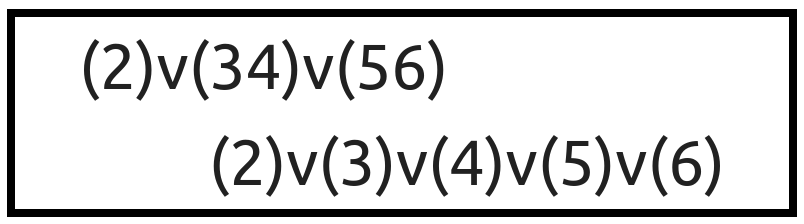
\includegraphics[scale=0.12]{images/x1/x1_5v_4e_2.png}
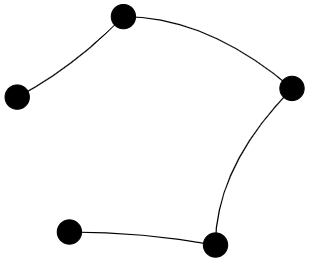
\includegraphics[scale=0.1]{images/x1/x1_5v_4e_2_vis.png}
\caption{$\mathcal{D}$-class of induced subgraph with 5 vertices and 4 edges (group C2).}
\end{figure}

\begin{figure}[H]
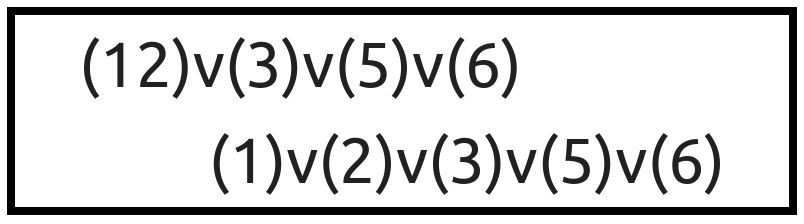
\includegraphics[scale=0.12]{images/x1/x1_5v_4e.png}
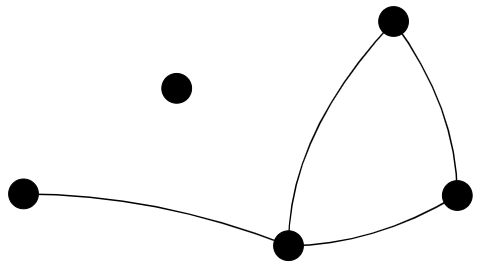
\includegraphics[scale=0.1]{images/x1/x1_5v_4e_1_vis.png}
\caption{$\mathcal{D}$-class of induced subgraph with 5 vertices and 4 edges (group C2).}
\end{figure}

\begin{figure}[H]
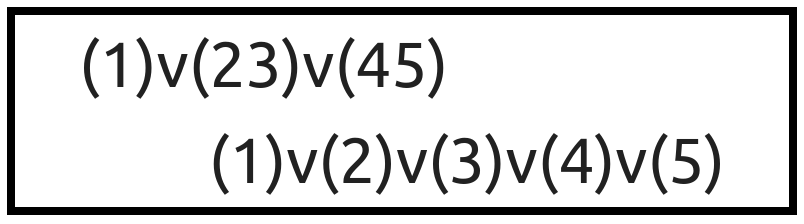
\includegraphics[scale=0.12]{images/x1/x1_5v_5e_2.png}
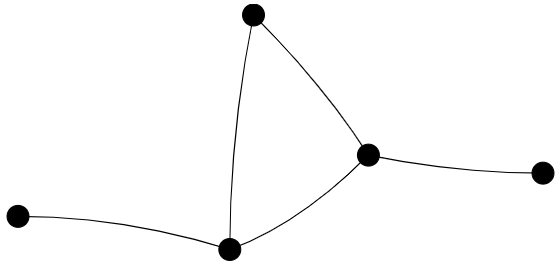
\includegraphics[scale=0.1]{images/x1/x1_5v_5e_2_vis.png}
\caption{$\mathcal{D}$-class of induced subgraph with 5 vertices and 5 edges (group C2).}
\end{figure}

\begin{figure}[H]
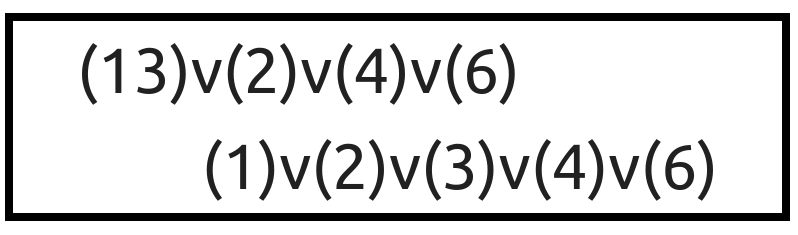
\includegraphics[scale=0.12]{images/x1/x1_5v_5e.png}
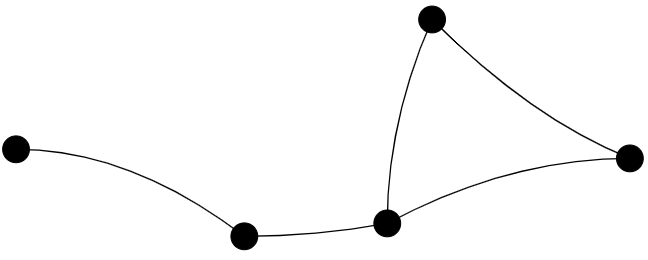
\includegraphics[scale=0.1]{images/x1/x1_5v_5e_1_vis.png}
\caption{$\mathcal{D}$-class of induced subgraph with 5 vertices and 5 edges (group C2).}
\end{figure}

\begin{figure}[H]
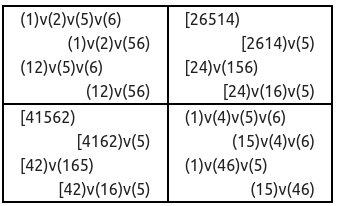
\includegraphics[scale=0.3]{images/x1/x1_4v_1e.png}
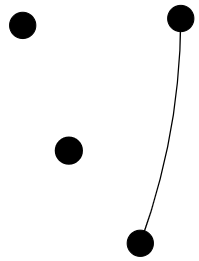
\includegraphics[scale=0.2]{images/x1/x1_4v_1e_vis.png}
\caption{$\mathcal{D}$-class of induced subgraph with 4 vertices and 1 edge (subgroup C2xC2).}
\end{figure}

\begin{figure}[H]
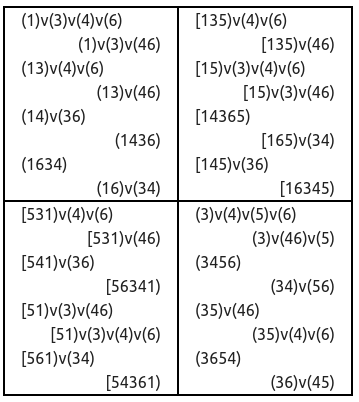
\includegraphics[scale=0.25]{images/x1/x1_4v_2e_2.png}
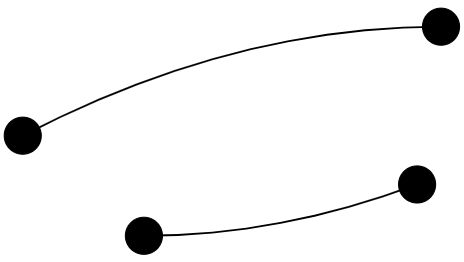
\includegraphics[scale=0.2]{images/x1/x1_4v_2e_2_vis.png}
\caption{$\mathcal{D}$-class of induced subgraph with 4 vertices and 2 edges (subgroup D8).}
\end{figure}

\begin{figure}[H]
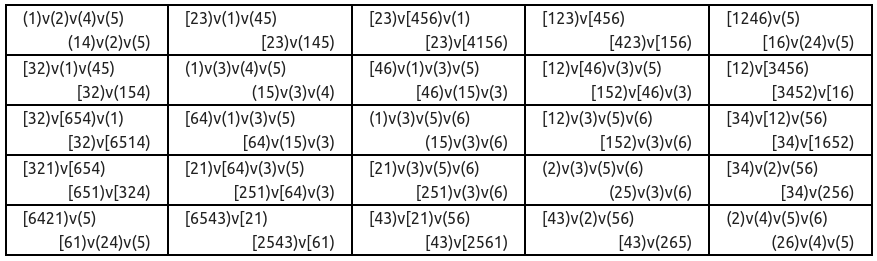
\includegraphics[scale=0.25]{images/x1/x1_4v_2e.png}
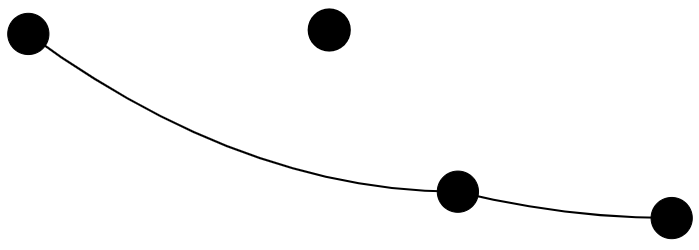
\includegraphics[scale=0.12]{images/x1/x1_4v_2e_1_vis.png}
\caption{$\mathcal{D}$-class of induced subgraph with 4 vertices and 2 edges (subgroup C2).}
\end{figure}

\begin{figure}[H]
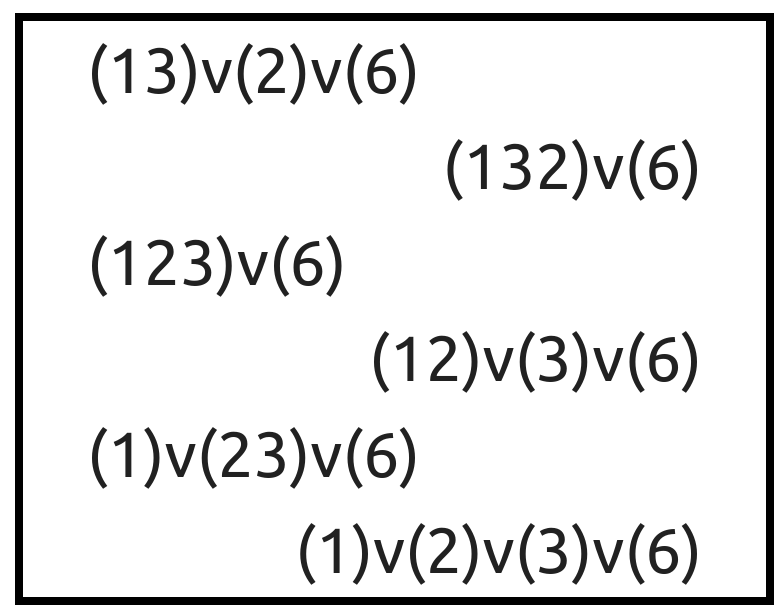
\includegraphics[scale=0.08]{images/x1/x1_4v_3e.png}
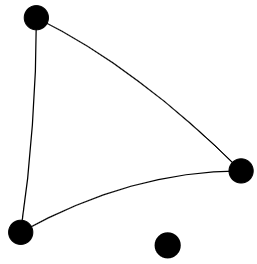
\includegraphics[scale=0.2]{images/x1/x1_4v_3e_1_vis.png}
\caption{$\mathcal{D}$-class of induced subgraph with 4 vertices and 3 edges (group S3).}
\end{figure}

\begin{figure}[H]
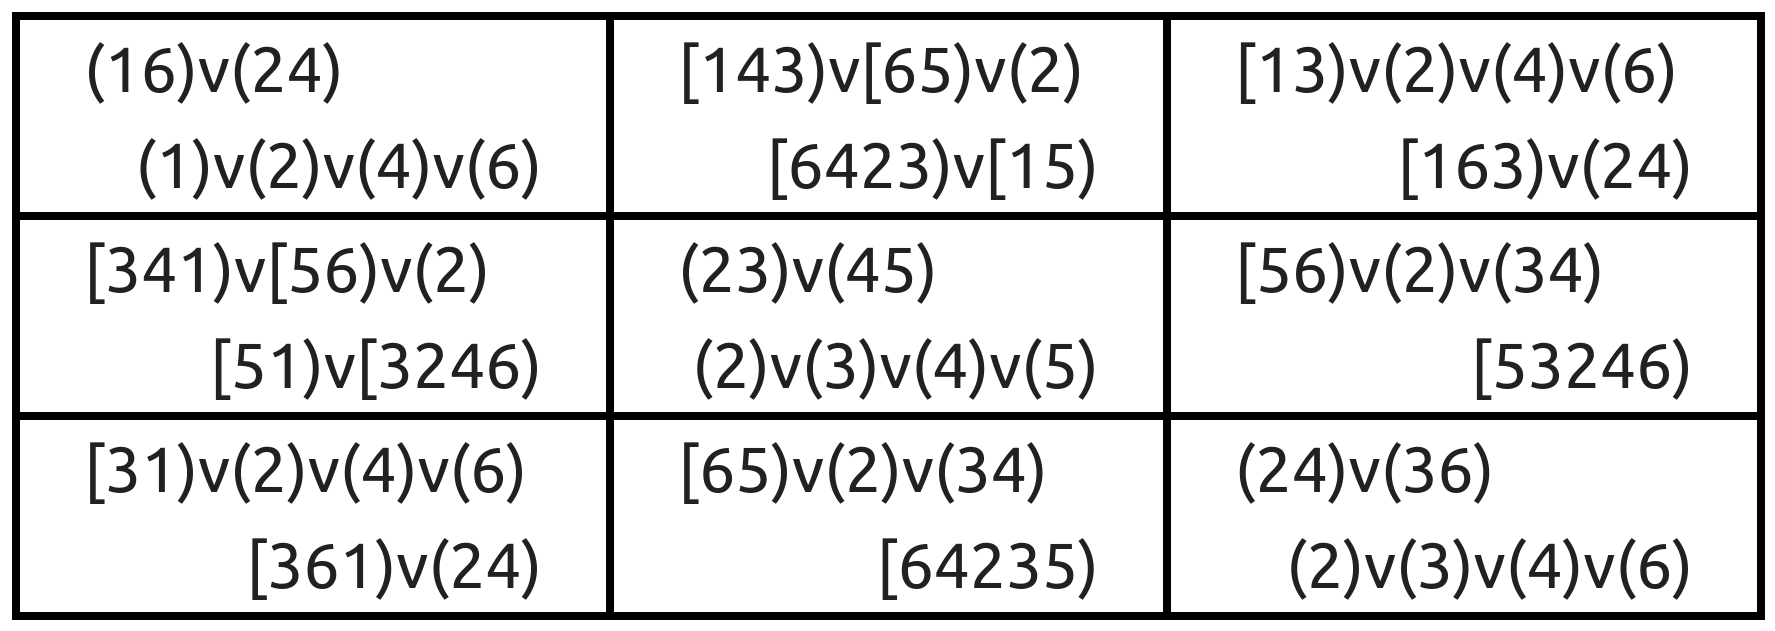
\includegraphics[scale=0.08]{images/x1/x1_4v_3e_2.png}
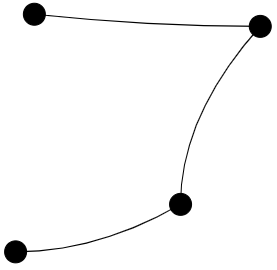
\includegraphics[scale=0.2]{images/x1/x1_4v_3e_2_vis.png}
\caption{$\mathcal{D}$-class of induced subgraph with 4 vertices and 3 edges (subgroup C2).}
\end{figure}

\begin{figure}[H]
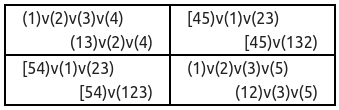
\includegraphics[scale=0.3]{images/x1/x1_4v_4e.png}
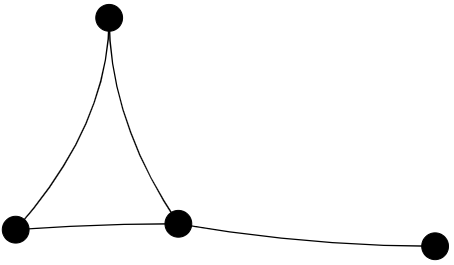
\includegraphics[scale=0.17]{images/x1/x1_4v_4e_vis.png}
\caption{$\mathcal{D}$-class of induced subgraph with 4 vertices and 4 edges (subgroup C2).}
\end{figure}

\begin{figure}[H]
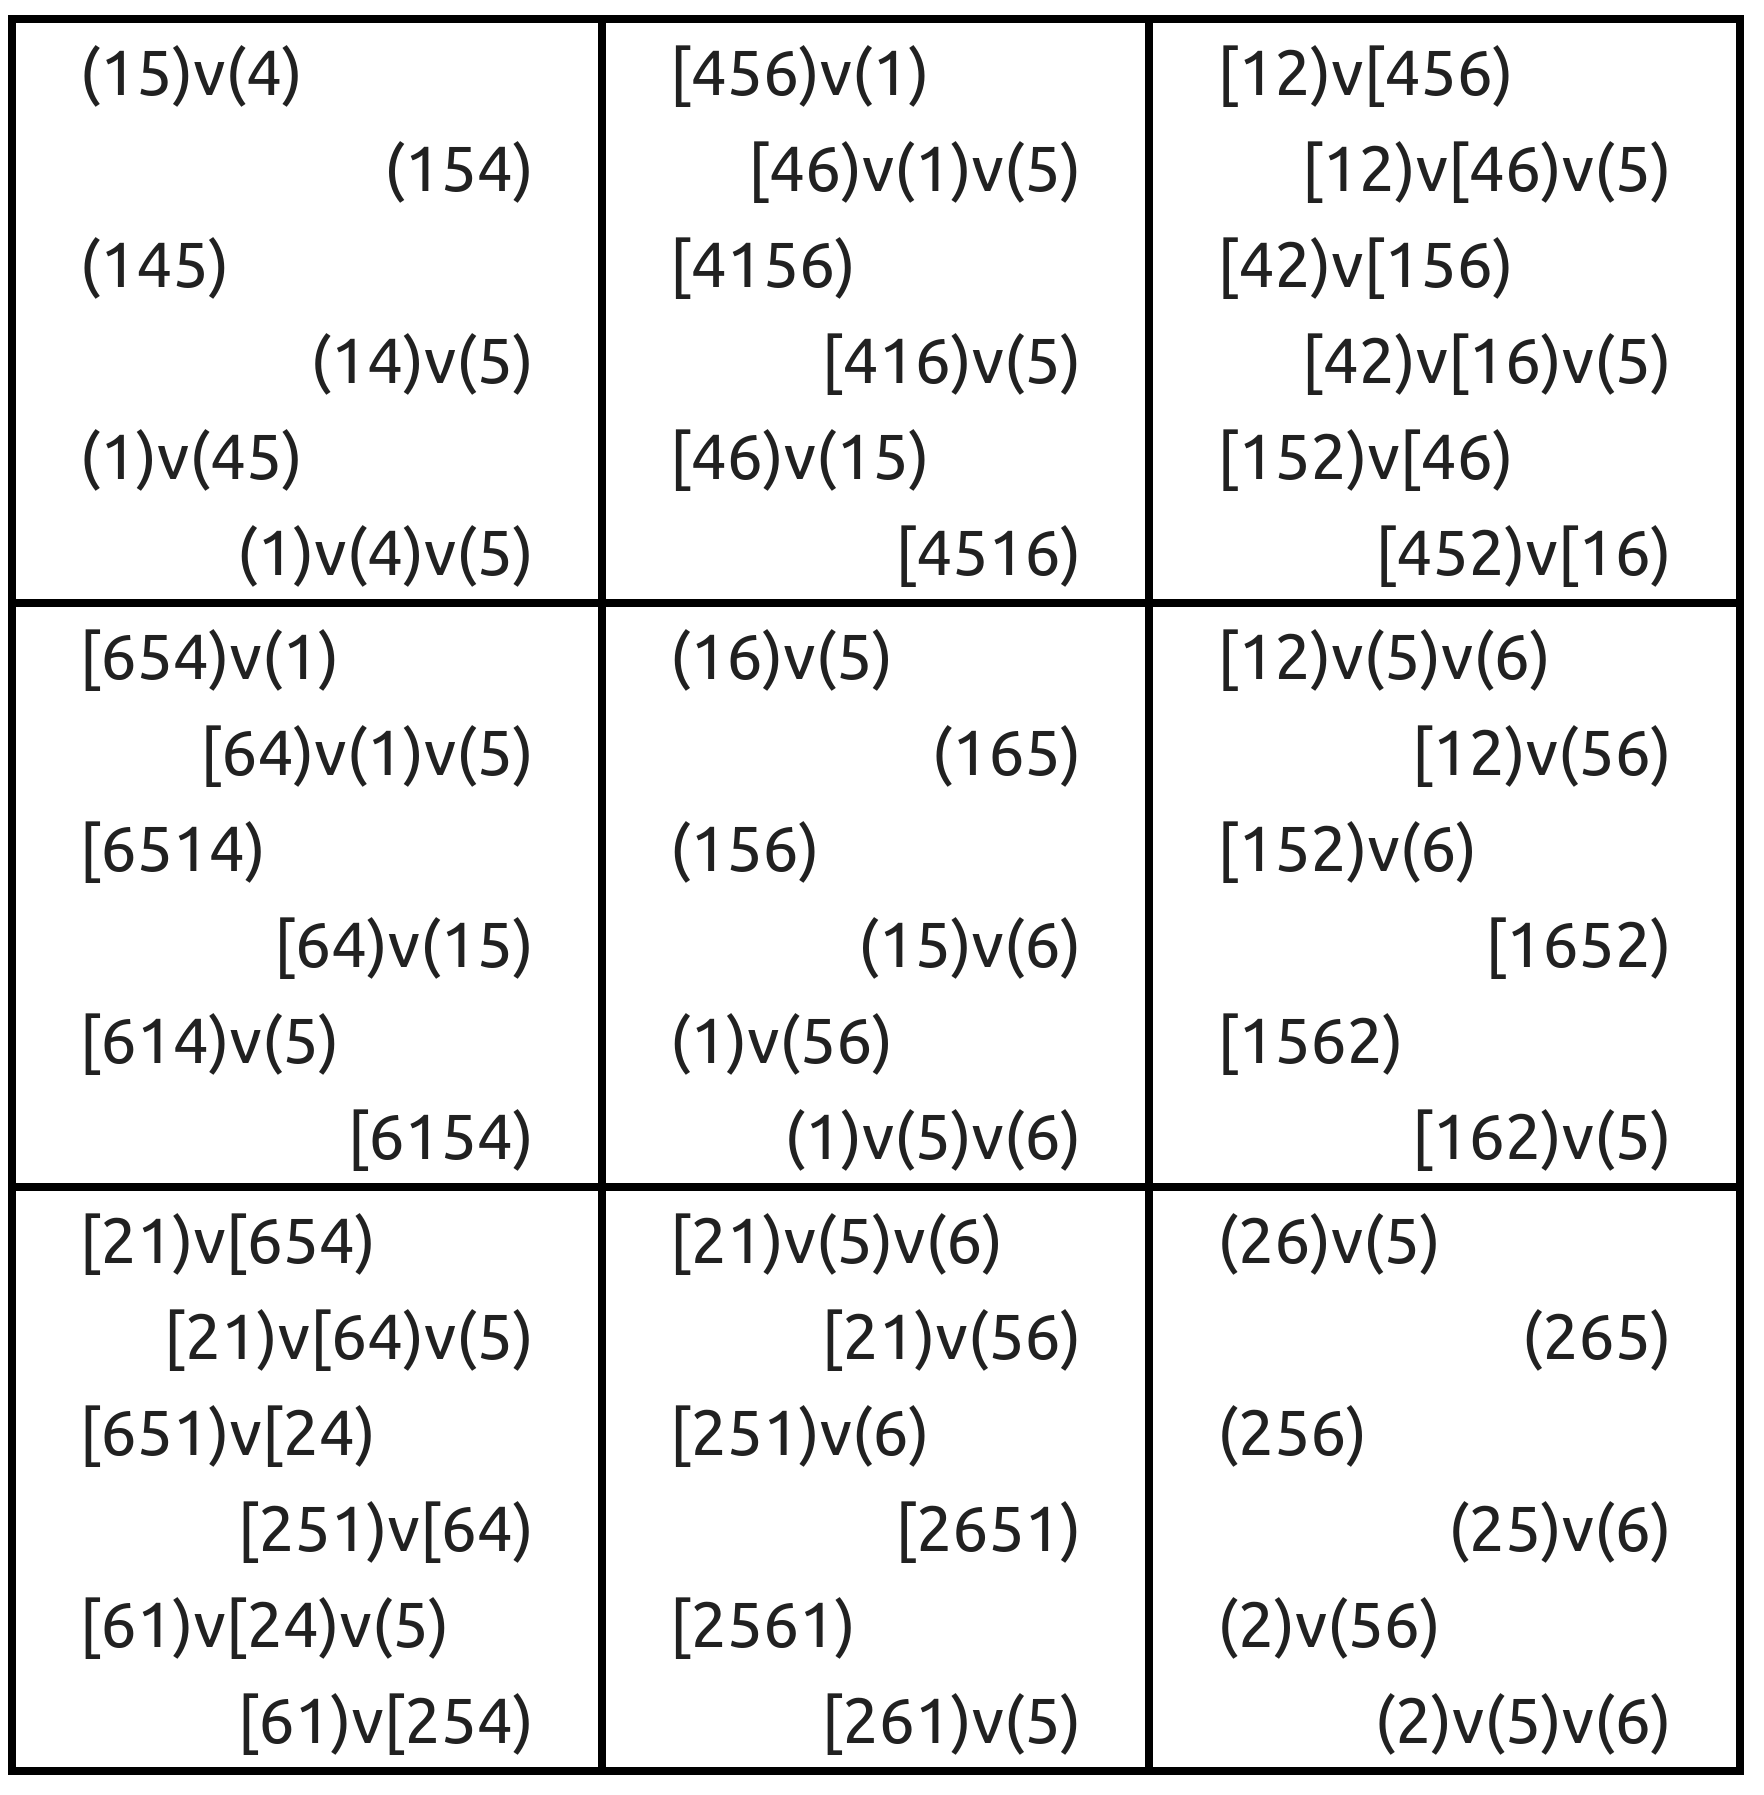
\includegraphics[scale=0.05]{images/x1/x1_3v_0e.png}
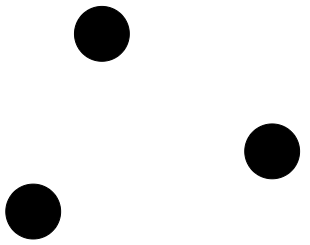
\includegraphics[scale=0.2]{images/x1/x1_3v_0e_vis.png}
\caption{$\mathcal{D}$-class of induced subgraph with 3 vertices and 0 edges (subgroup S3).}
\end{figure}

\begin{figure}[H]
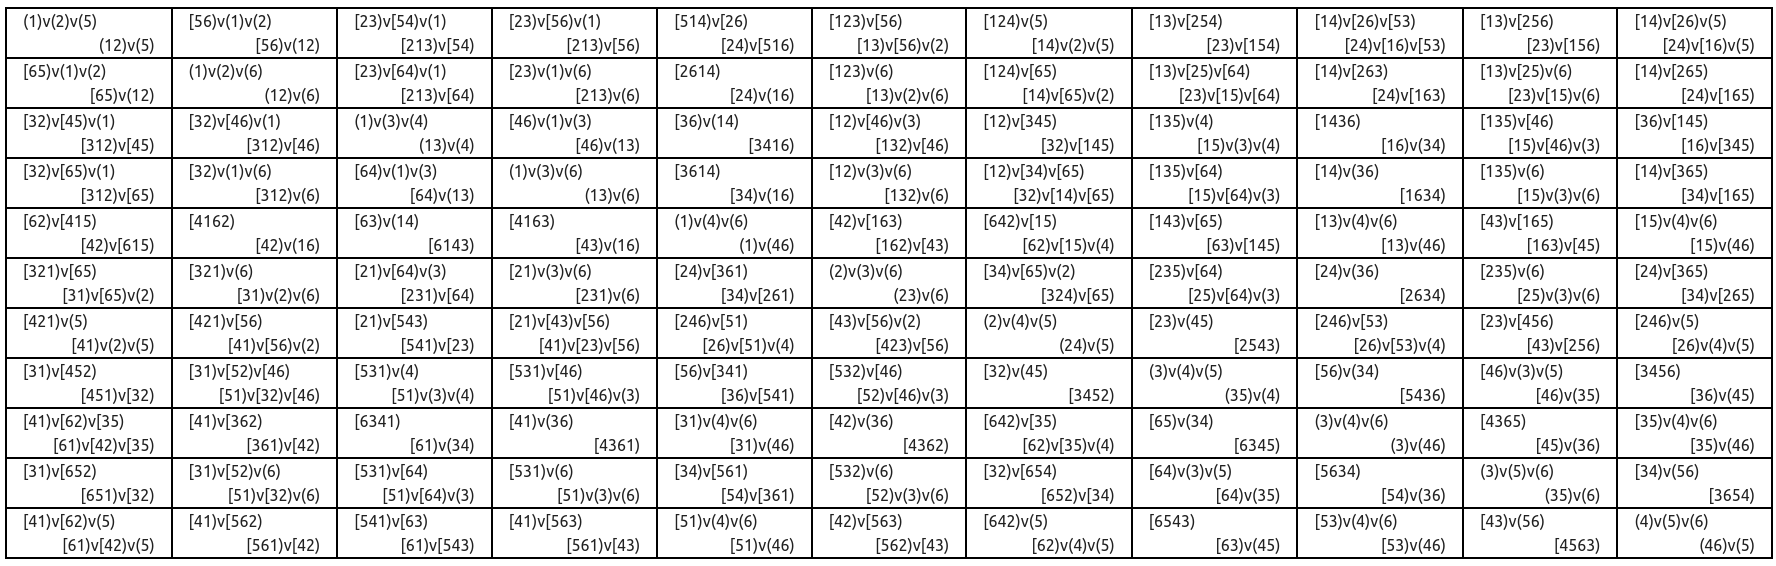
\includegraphics[width=\textwidth, keepaspectratio]{images/x1/x1_3v_1e.png}
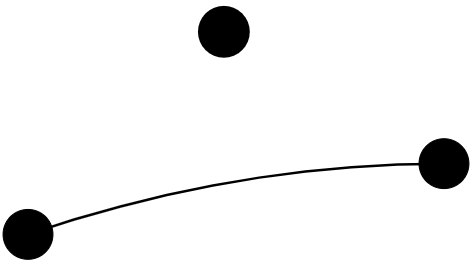
\includegraphics[scale=0.15]{images/x1/x1_3v_1e_vis.png}
\caption{$\mathcal{D}$-class of induced subgraph with 3 vertices and 1 edge (subgroup C2).}
\end{figure}

\begin{figure}[H]
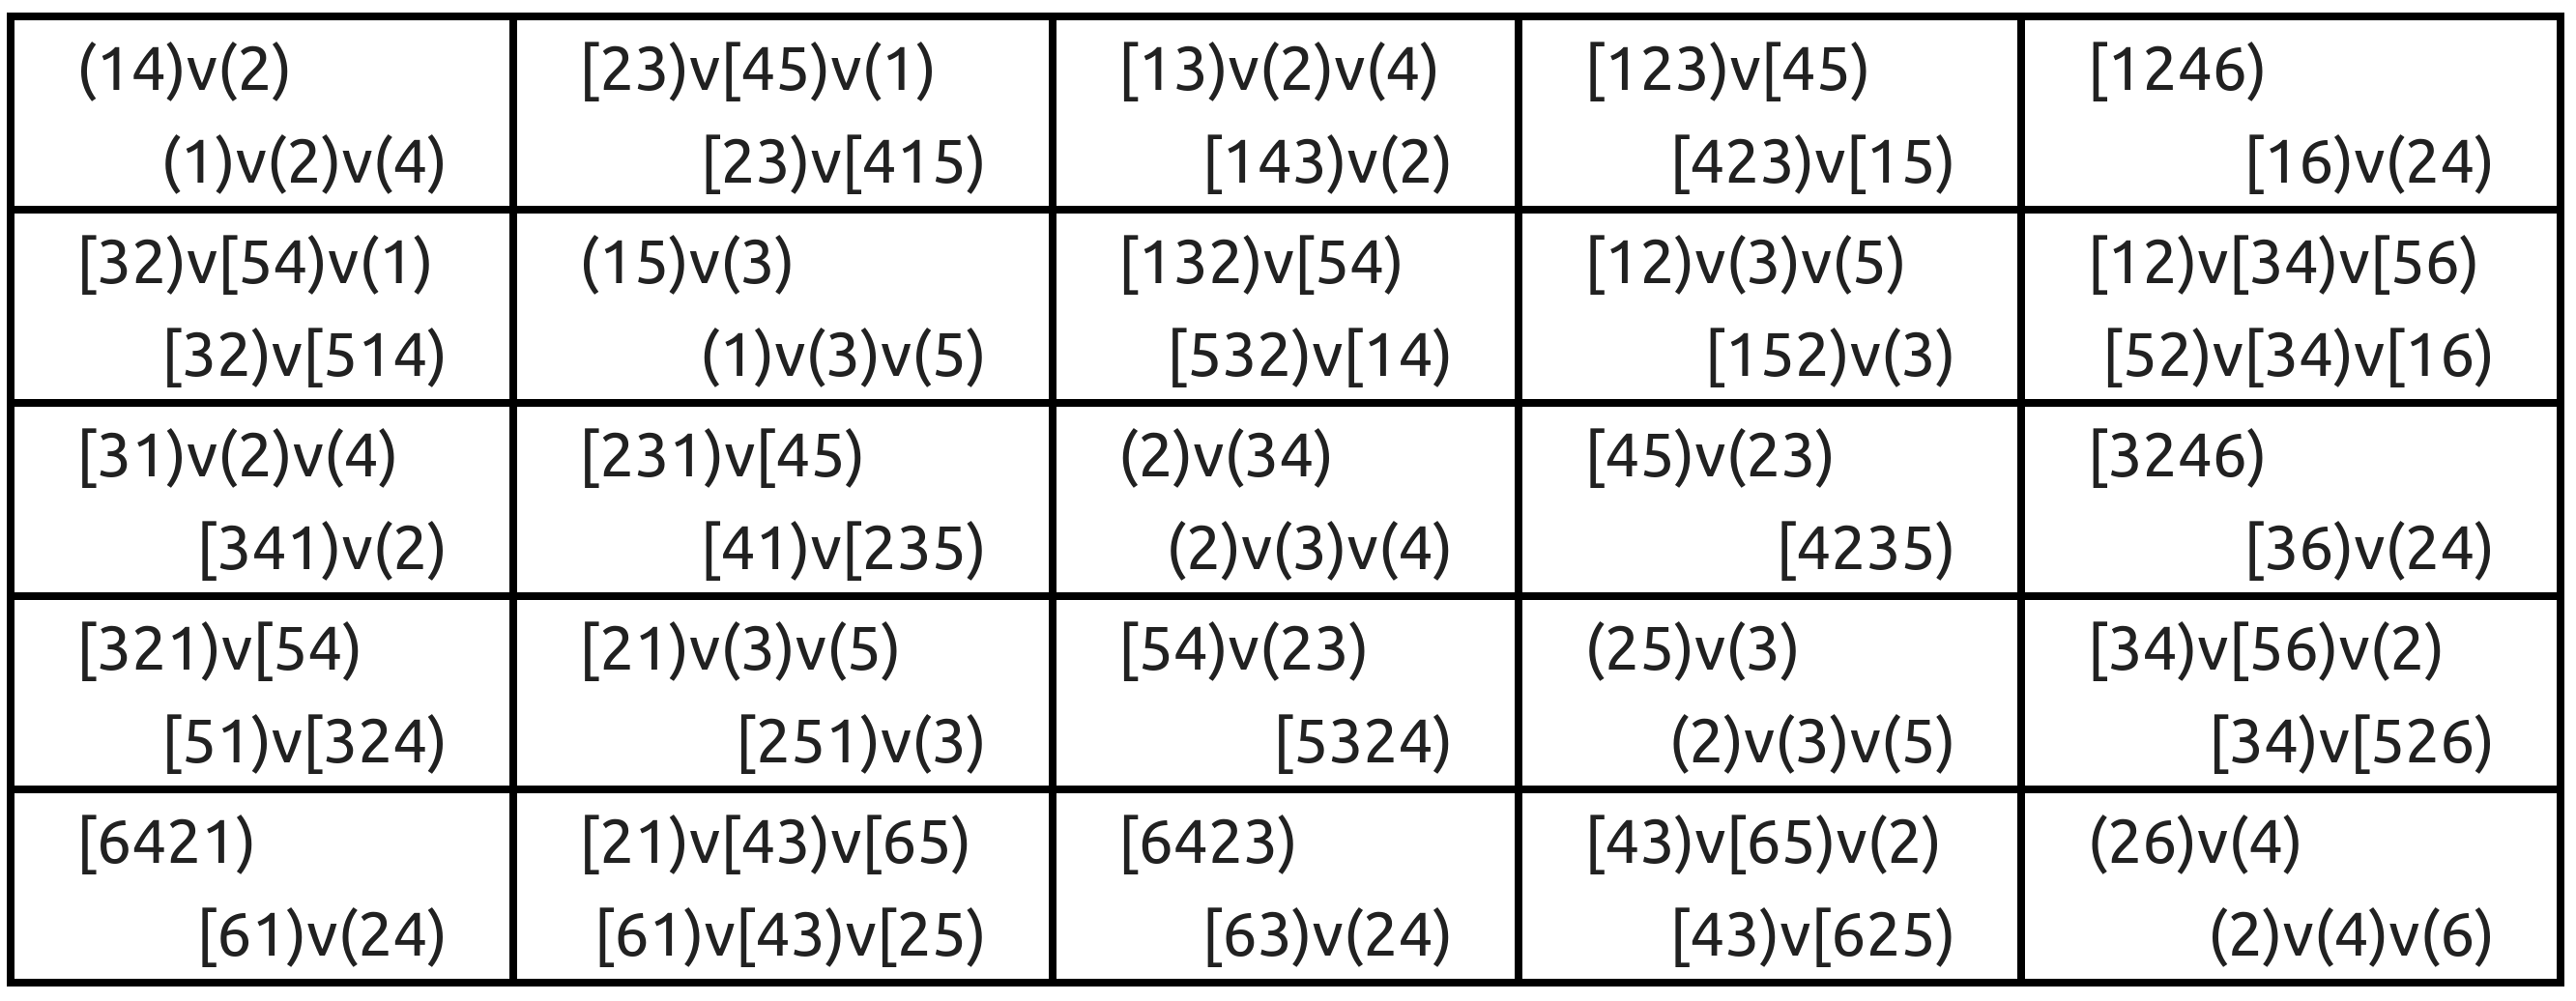
\includegraphics[scale=0.08]{images/x1/x1_3v_2e.png}
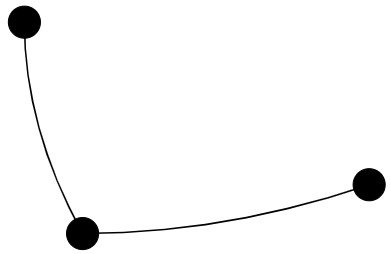
\includegraphics[scale=0.12]{images/x1/x1_3v_2e_vis.png}
\caption{$\mathcal{D}$-class of induced subgraph with 3 vertices and 2 edges (subgroup C2).}
\end{figure}

\begin{figure}[H]
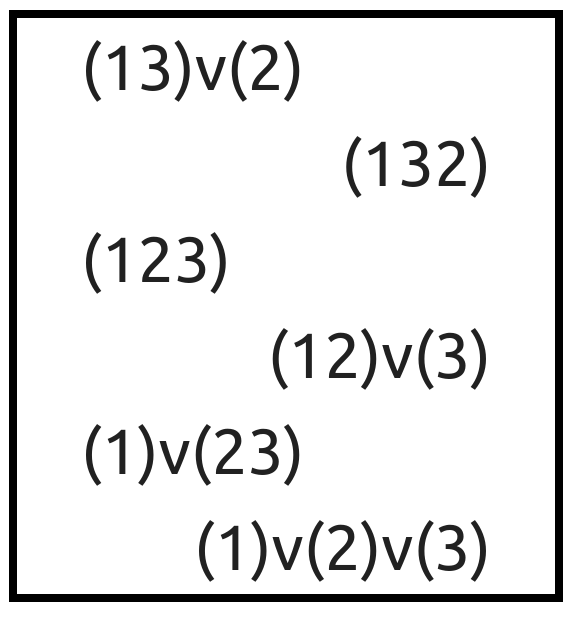
\includegraphics[scale=0.08]{images/x1/x1_3v_3e.png}
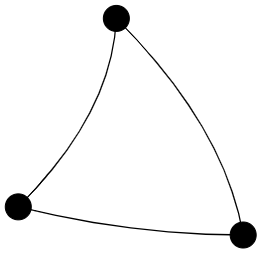
\includegraphics[scale=0.15]{images/x1/x1_3v_3e_vis.png}
\caption{$\mathcal{D}$-class of induced subgraph with 3 vertices and 3 edges (group S3).}
\end{figure}

\begin{figure}[H]
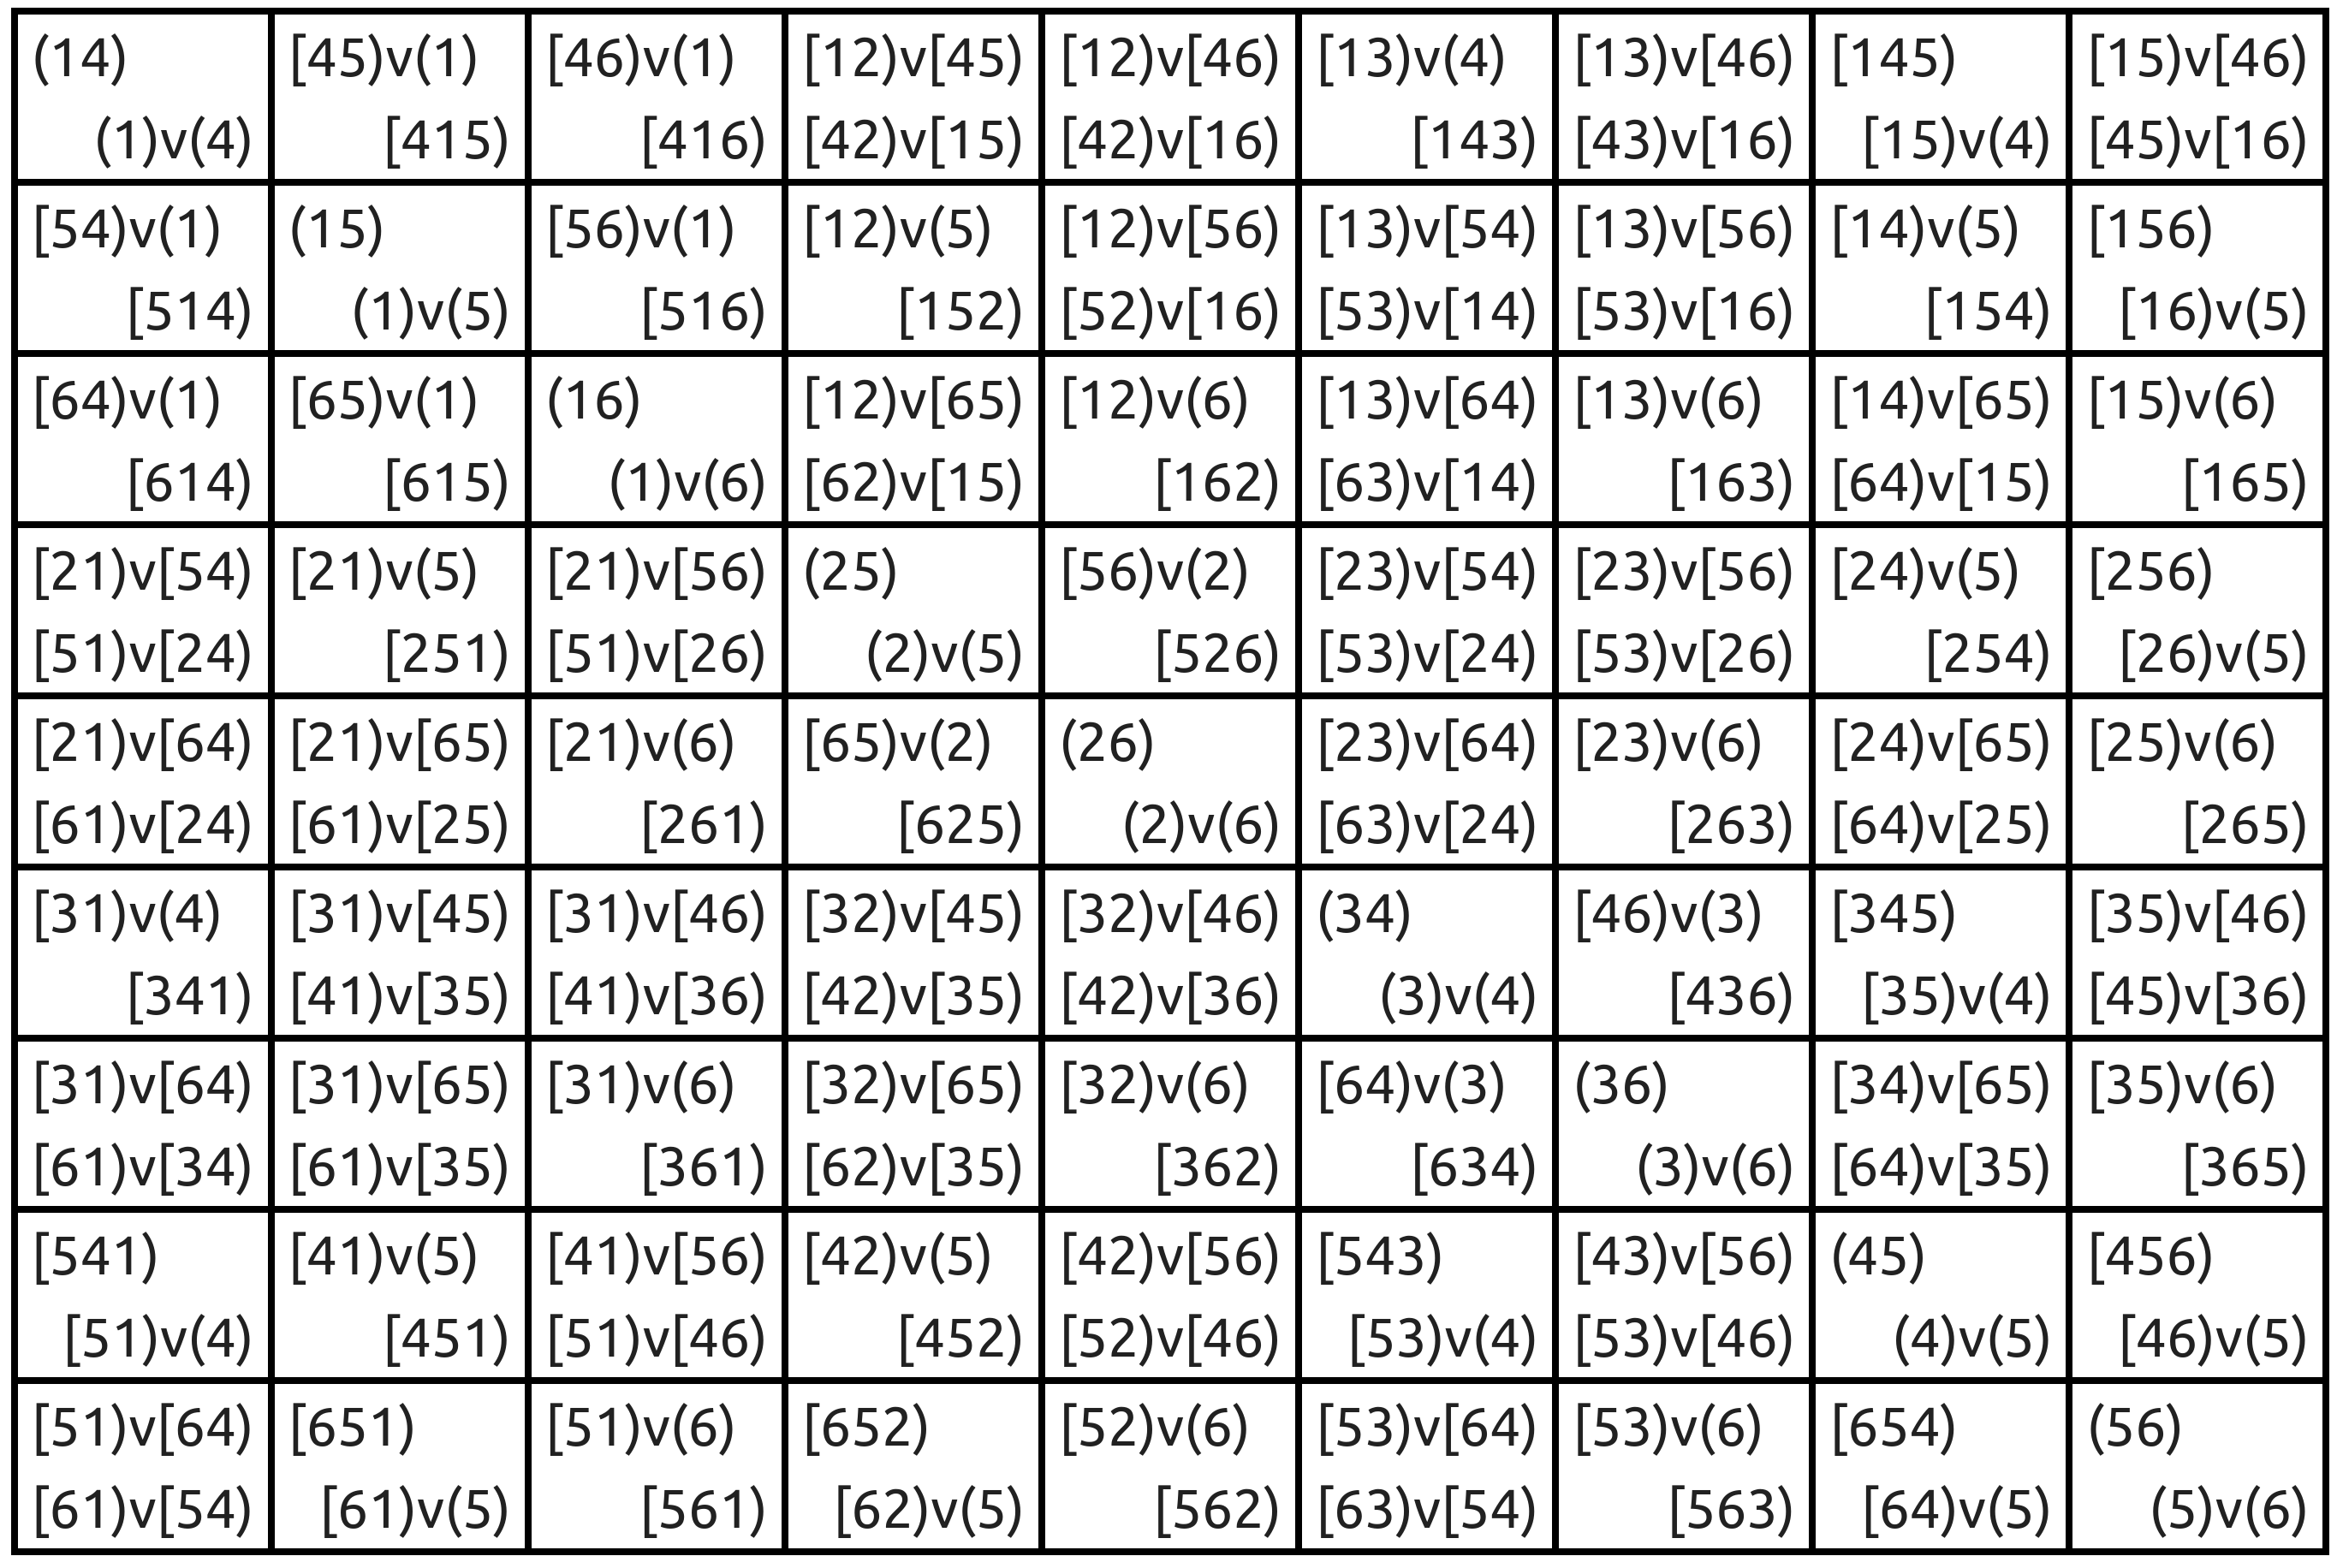
\includegraphics[scale=0.08]{images/x1/x1_2v_0e.png}
\caption{$\mathcal{D}$-class of induced subgraph with 2 vertices and 0 edges (subgroup C2).}
\end{figure}

\begin{figure}[H]
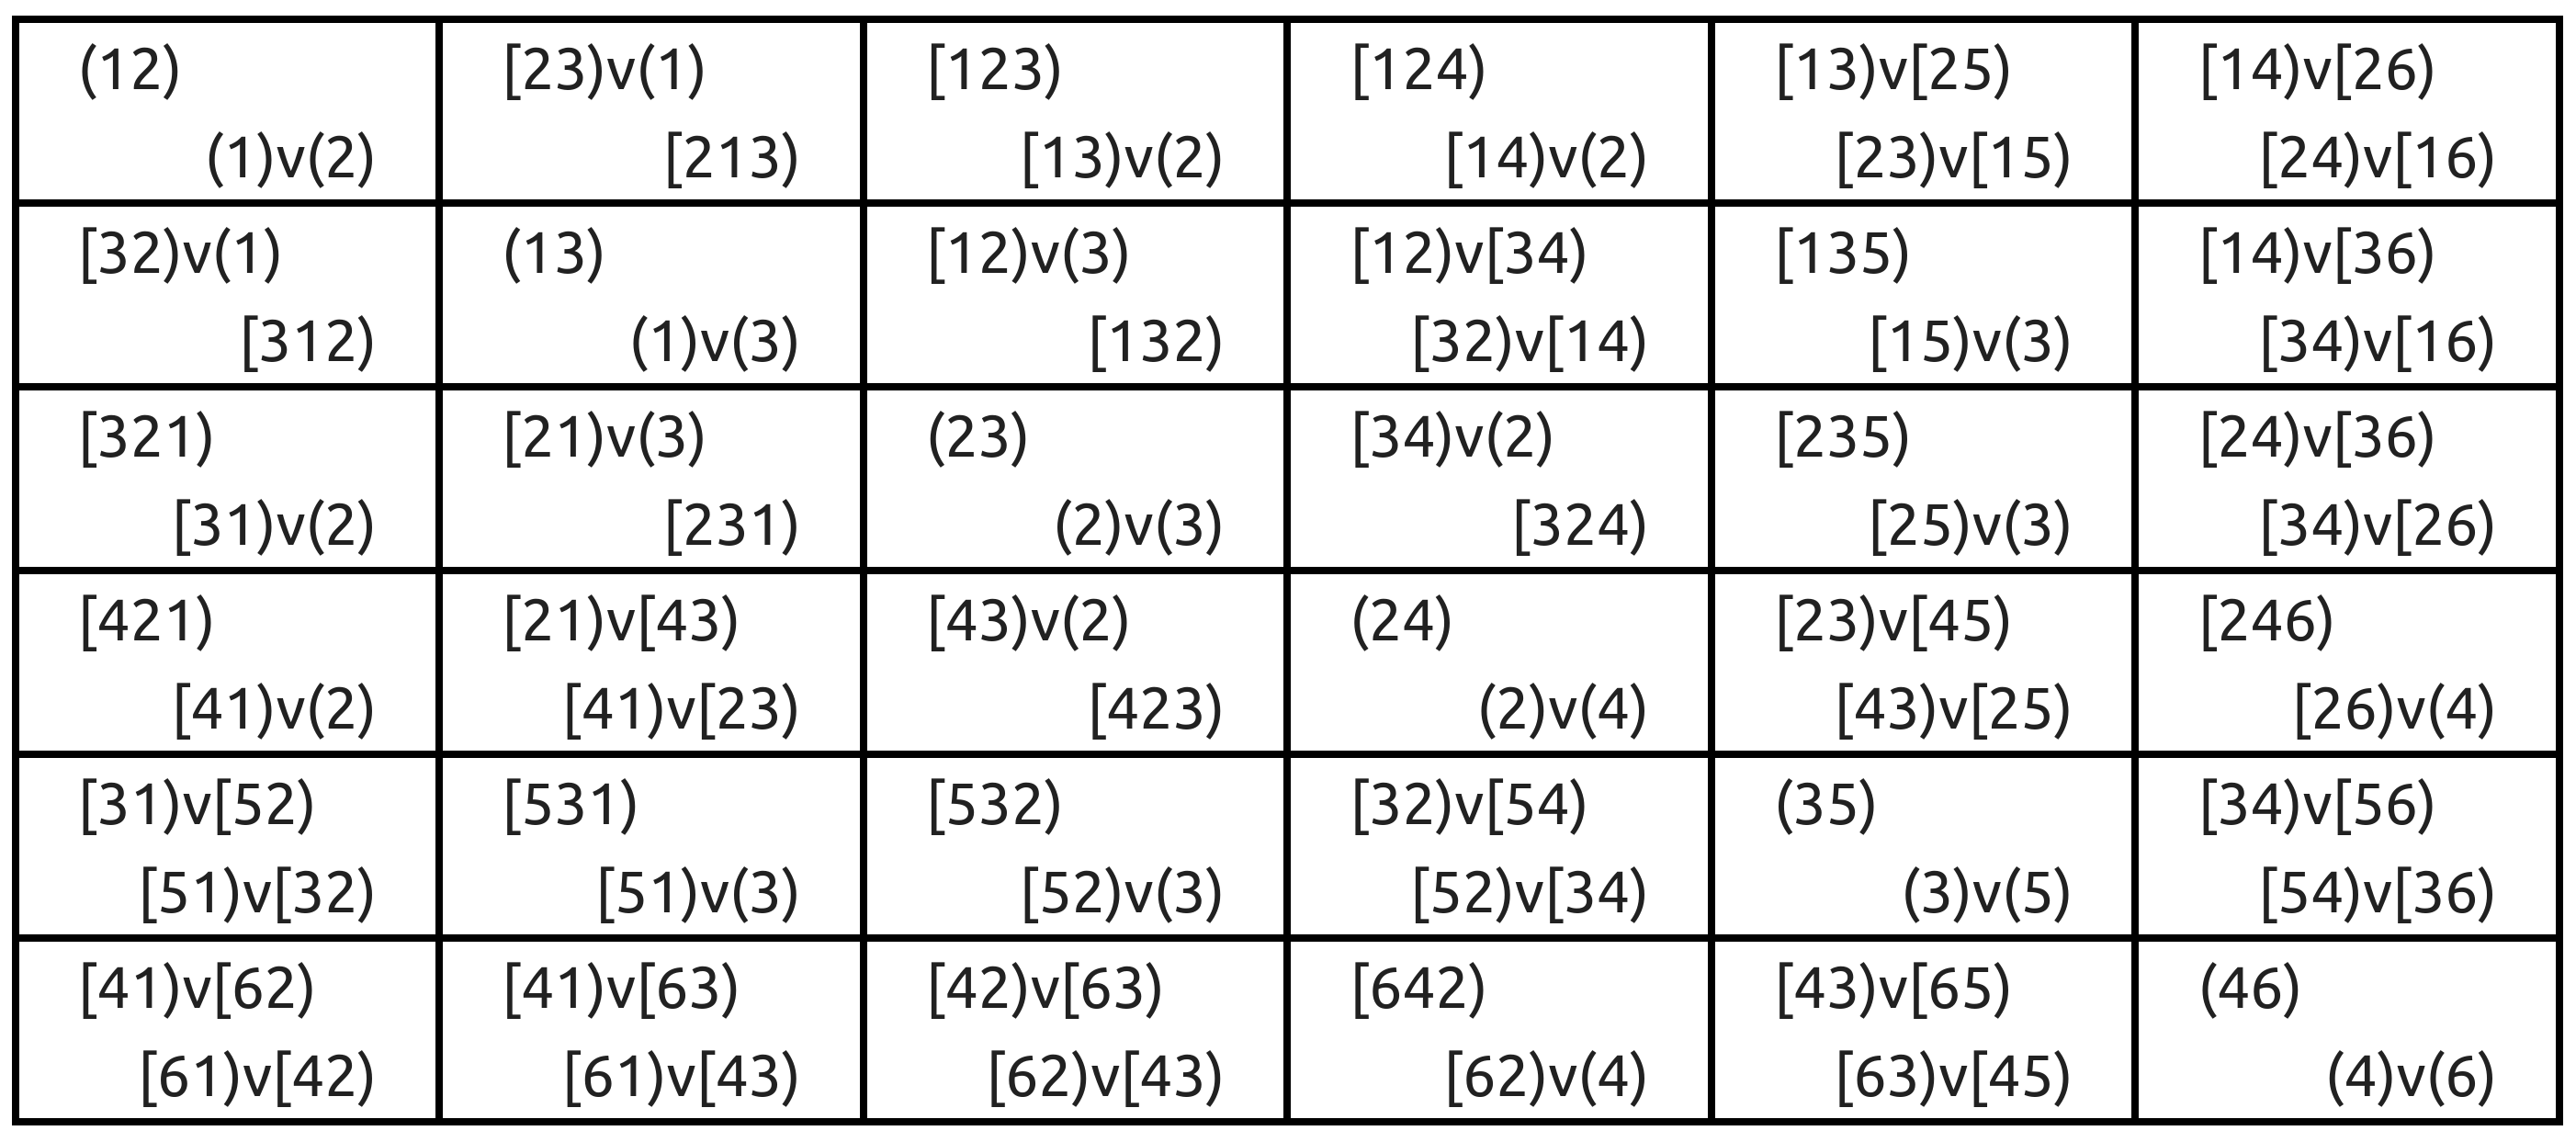
\includegraphics[scale=0.06]{images/x1/x1_2v_1e.png}
\caption{$\mathcal{D}$-class of induced subgraph with 2 vertices and 1 edge (subgroup C2).}
\end{figure}

\begin{figure}[H]
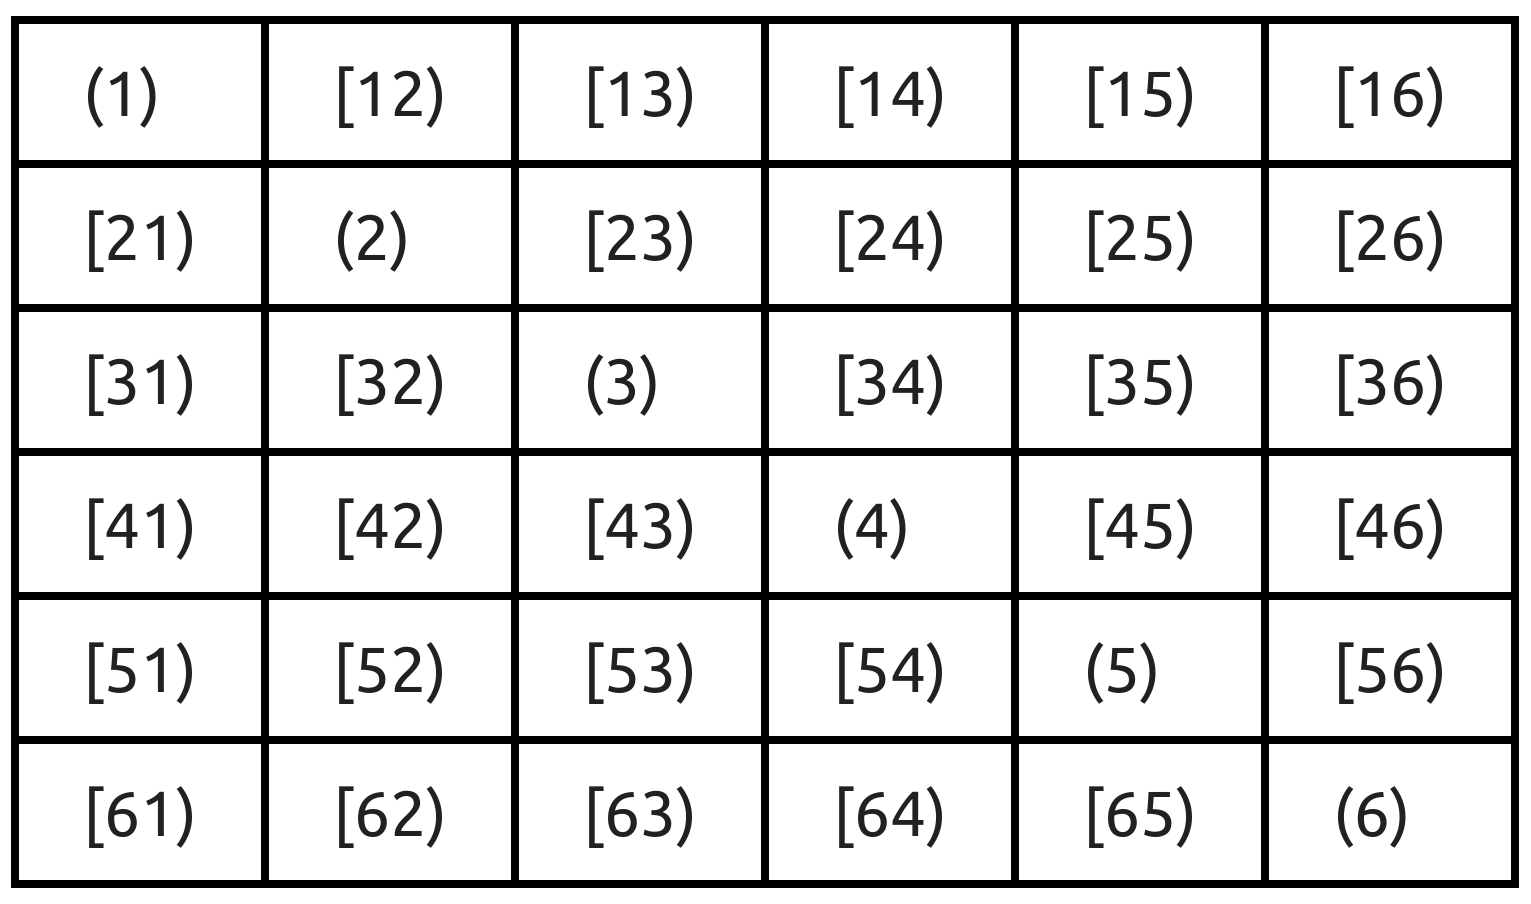
\includegraphics[scale=0.06]{images/x1/x1_1v_0e.png}
\caption{$\mathcal{D}$-class of induced subgraph with 1 vertex and 0 edges.}
\end{figure}

\section{Partial automorphism monoid of minimal asymmetric graph X9}

\begin{figure}[H]
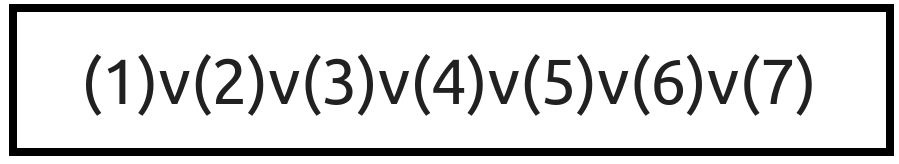
\includegraphics[scale=0.1]{images/x9/x9_7v_6e.png}
\caption{$\mathcal{D}$-class of induced subgraph with 7 vertices and 6 edges.}
\end{figure}

\begin{figure}[H]
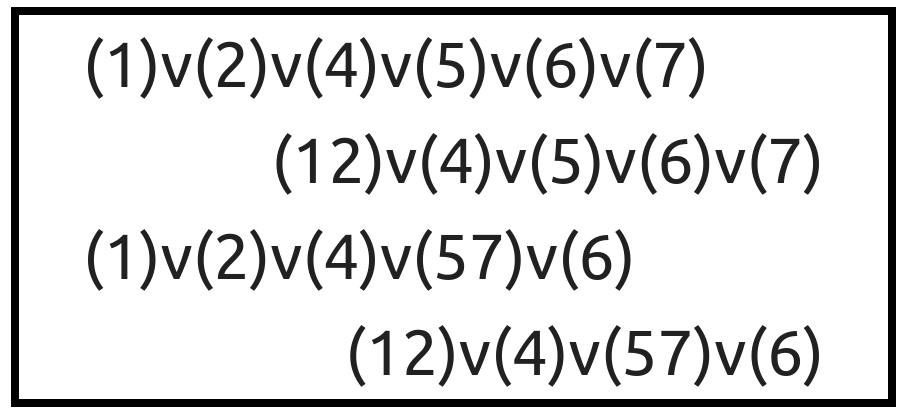
\includegraphics[scale=0.1]{images/x9/x9_6v_3e.png}
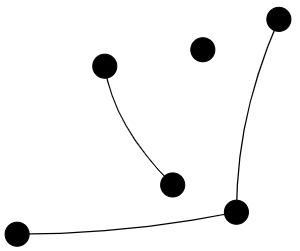
\includegraphics[scale=0.15]{images/x9/x9_6v_3e_vis.png}
\caption{$\mathcal{D}$-class of induced subgraph with 6 vertices and 3 edges (group C2xC2).}
\end{figure}

\begin{figure}[H]
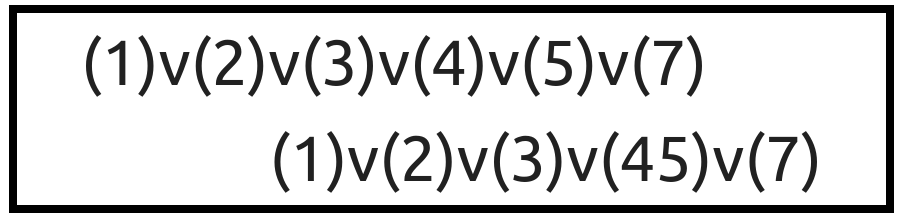
\includegraphics[scale=0.1]{images/x9/x9_6v_4e_1.png}
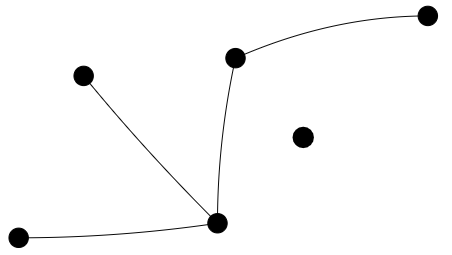
\includegraphics[scale=0.15]{images/x9/x9_6v_4e_1_vis.png}
\caption{$\mathcal{D}$-class of induced subgraph with 6 vertices and 4 edges (group C2).}
\end{figure}

\begin{figure}[H]
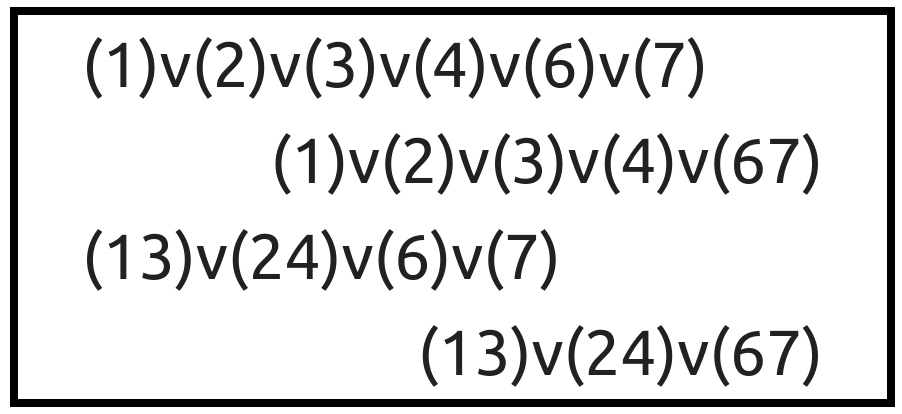
\includegraphics[scale=0.1]{images/x9/x9_6v_4e_2.png}
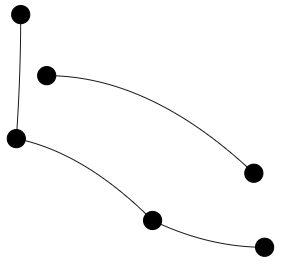
\includegraphics[scale=0.15]{images/x9/x9_6v_4e_2_vis.png}
\caption{$\mathcal{D}$-class of induced subgraph with 6 vertices and 4 edges (group C2xC2).}
\end{figure}

\begin{figure}[H]
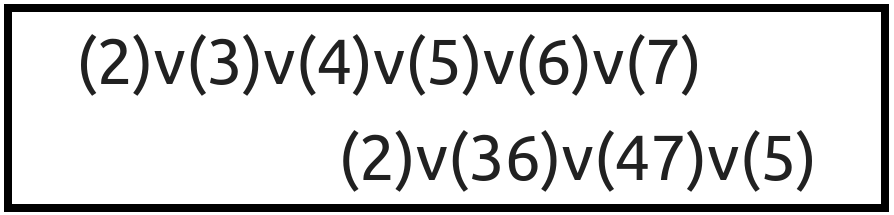
\includegraphics[scale=0.1]{images/x9/x9_6v_4e_3.png}
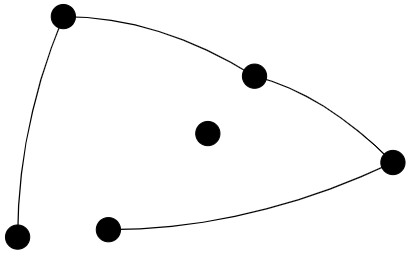
\includegraphics[scale=0.1]{images/x9/x9_6v_4e_3_vis.png}
\caption{$\mathcal{D}$-class of induced subgraph with 6 vertices and 4 edges (group C2).}
\end{figure}

\begin{figure}[H]
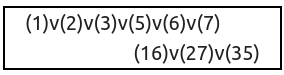
\includegraphics[scale=0.35]{images/x9/x9_6v_5e_1.png}
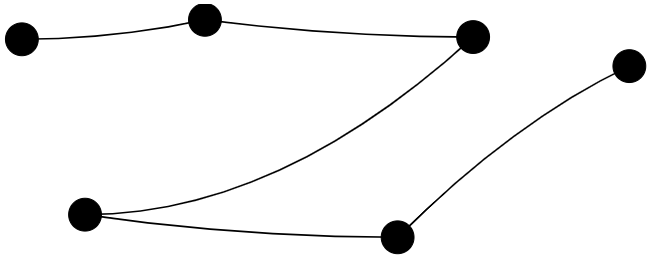
\includegraphics[scale=0.1]{images/x9/x9_6v_5e_1_vis.png}
\caption{$\mathcal{D}$-class of induced subgraph with 6 vertices and 5 edges (group C2).}
\end{figure}

\begin{figure}[H]
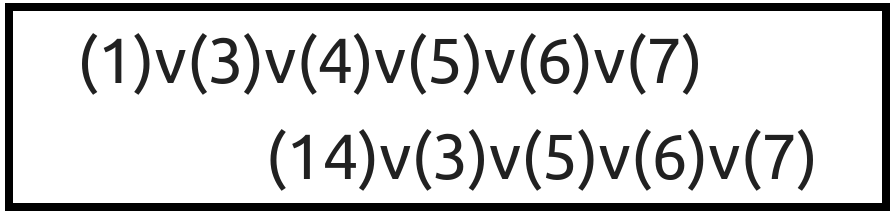
\includegraphics[scale=0.14]{images/x9/x9_6v_5e_2.png}
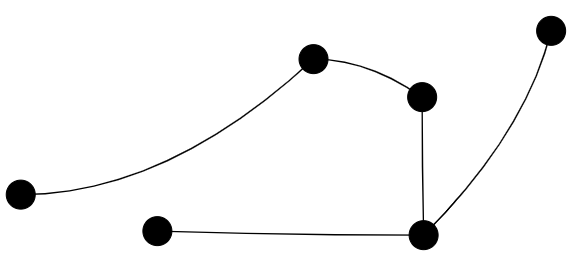
\includegraphics[scale=0.08]{images/x9/x9_6v_5e_2_vis.png}
\caption{$\mathcal{D}$-class of induced subgraph with 6 vertices and 5 edges (group C2).}
\end{figure}

\begin{figure}[H]
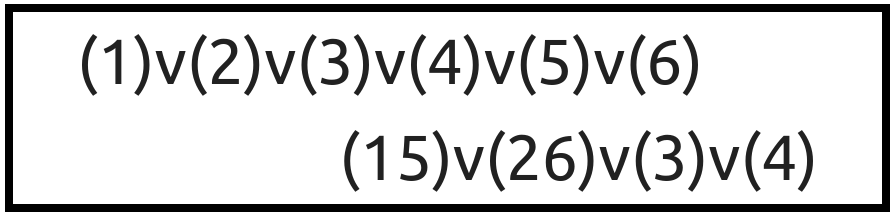
\includegraphics[scale=0.14]{images/x9/x9_6v_5e_3.png}
\includegraphics[scale=0.1]{images/x9/x9_6v_5e_3_vis.png}
\caption{$\mathcal{D}$-class of induced subgraph with 6 vertices and 5 edges (group C2).}
\end{figure}

\begin{figure}[H]
\includegraphics[scale=0.09]{images/x9/x9_5v_1e.png}
\includegraphics[scale=0.1]{images/x9/x9_5v_1e_vis.png}
\caption{$\mathcal{D}$-class of induced subgraph with 5 vertices and 1 edge (group D12).}
\end{figure}

\begin{figure}[H]
\includegraphics[scale=0.2]{images/x9/x9_5v_2e_1.png}
\includegraphics[scale=0.1]{images/x9/x9_5v_2e_1_vis.png}
\caption{$\mathcal{D}$-class of induced subgraph with 5 vertices and 2 edges (subgroup C2xC2).}
\end{figure}

\begin{figure}[H]
\includegraphics[scale=0.25]{images/x9/x9_5v_2e_2.png}
\includegraphics[scale=0.1]{images/x9/x9_5v_2e_2_vis.png}
\caption{$\mathcal{D}$-class of induced subgraph with 5 vertices and 2 edges (subgroup C2).}
\end{figure}

\begin{figure}[H]
\includegraphics[scale=0.09]{images/x9/x9_5v_3e_1.png}
\includegraphics[scale=0.1]{images/x9/x9_5v_3e_1_vis.png}
\caption{$\mathcal{D}$-class of induced subgraph with 5 vertices and 3 edges (group S3).}
\end{figure}

\begin{figure}[H]
\includegraphics[scale=0.2]{images/x9/x9_5v_3e_2.png}
\includegraphics[scale=0.1]{images/x9/x9_5v_3e_2_vis.png}
\caption{$\mathcal{D}$-class of induced subgraph with 5 vertices and 3 edges (subgroup C2xC2).}
\end{figure}

\begin{figure}[H]
\includegraphics[scale=0.2]{images/x9/x9_5v_3e_3.png}
\includegraphics[scale=0.1]{images/x9/x9_5v_3e_3_vis.png}
\caption{$\mathcal{D}$-class of induced subgraph with 5 vertices and 3 edges (subgroup C2).}
\end{figure}

\begin{figure}[H]
\includegraphics[scale=0.25]{images/x9/x9_5v_4e_1.png}
\includegraphics[scale=0.1]{images/x9/x9_5v_4e_1_vis.png}
\caption{$\mathcal{D}$-class of induced subgraph with 5 vertices and 4 edges (subgroup C2).}
\end{figure}

\begin{figure}[H]
\includegraphics[scale=0.25]{images/x9/x9_5v_4e_2.png}
\includegraphics[scale=0.1]{images/x9/x9_5v_4e_2_vis.png}
\caption{$\mathcal{D}$-class of induced subgraph with 5 vertices and 4 edges (subgroup C2).}
\end{figure}

\begin{figure}[H]
\includegraphics[scale=0.15]{images/x9/x9_4v_0e.png}
\includegraphics[scale=0.1]{images/x9/x9_4v_0e_vis.png}
\caption{$\mathcal{D}$-class of induced subgraph with 4 vertices and 0 edges (subgroup S4).}
\end{figure}

\begin{figure}[H]
\includegraphics[width=\textwidth,keepaspectratio]{images/x9/x9_4v_1e.png}
\includegraphics[scale=0.1]{images/x9/x9_4v_1e_vis.png}
\caption{$\mathcal{D}$-class of induced subgraph with 4 vertices and 1 edge (subgroup C2xC2).}
\end{figure}

\begin{figure}[H]
\includegraphics[scale=0.1]{images/x9/x9_4v_2e_1.png}
\includegraphics[scale=0.1]{images/x9/x9_4v_2e_1_vis.png}
\caption{$\mathcal{D}$-class of induced subgraph with 4 vertices and 2 edges (subgroup D8).}
\end{figure}

\begin{figure}[H]
\includegraphics[width=\textwidth,keepaspectratio]{images/x9/x9_4v_2e_2.png}
\includegraphics[scale=0.1]{images/x9/x9_4v_2e_2_vis.png}
\caption{$\mathcal{D}$-class of induced subgraph with 4 vertices and 2 edges (subgroup C2).}
\end{figure}

\begin{figure}[H]
\includegraphics[scale=0.1]{images/x9/x9_4v_3e_1.png}
\includegraphics[scale=0.1]{images/x9/x9_4v_3e_1_vis.png}
\caption{$\mathcal{D}$-class of induced subgraph with 4 vertices and 3 edges (group S3).}
\end{figure}

\begin{figure}[H]
\includegraphics[scale=0.2]{images/x9/x9_4v_3e_2.png}
\includegraphics[scale=0.1]{images/x9/x9_4v_3e_2_vis.png}
\caption{$\mathcal{D}$-class of induced subgraph with 4 vertices and 3 edges (subgroup C2).}
\end{figure}

\begin{figure}[H]
\includegraphics[width=\textwidth,keepaspectratio]{images/x9/x9_3v_0e.png}
\includegraphics[scale=0.1]{images/x1/x1_3v_0e_vis.png}
\caption{$\mathcal{D}$-class of induced subgraph with 3 vertices and 0 edges (subgroup S3).}
\end{figure}

\begin{figure}[H]
\includegraphics[width=\textwidth,keepaspectratio]{images/x9/x9_3v_1e.png}
\includegraphics[scale=0.1]{images/x1/x1_3v_1e_vis.png}
\caption{$\mathcal{D}$-class of induced subgraph with 3 vertices and 1 edge (subgroup C2).}
\end{figure}

\begin{figure}[H]
\includegraphics[scale=0.15]{images/x9/x9_3v_2e.png}
\includegraphics[scale=0.1]{images/x1/x1_3v_2e_vis.png}
\caption{$\mathcal{D}$-class of induced subgraph with 3 vertices and 2 edges (subgroup C2).}
\end{figure}

\begin{figure}[H]
\includegraphics[width=\textwidth, keepaspectratio]{images/x9/x9_2v_0e.png}
\caption{$\mathcal{D}$-class of induced subgraph with 2 vertices and 0 edges (subgroup C2).}
\end{figure}

\begin{figure}[H]
\includegraphics[scale=0.15]{images/x9/x9_2v_1e.png}
\caption{$\mathcal{D}$-class of induced subgraph with 2 vertices and 1 edge (subgroup C2).}
\end{figure}

\begin{figure}[H]
\includegraphics[scale=0.2]{images/x9/x9_1v_0e.png}
\caption{$\mathcal{D}$-class of induced subgraph with 1 vertex and 0 edges.}
\end{figure}

\end{appendices}